\chapter{Deliverable}
\label{chap:Deliverable}

This chapter will go through the work that was produced as a result of this
project. We will take a look at the website, examples of code for both frameworks,
and how we tested both frameworks.

\section{The Website - Wire}

Most of the features that we planned for were implemented in the final version
of the website. The website was named `Wire' and users can create an account,
post messages, follow other users, see user messages, post tagged
messages, and search for other messages and users. The following subsections
contain pictures of the website produced. The pictures taken are of the Yesod
website but the Django site is functionally identical, with only a few minor styling
differences.

\subsection{The Home Page}

\begin{figure}[H]
    \centering
    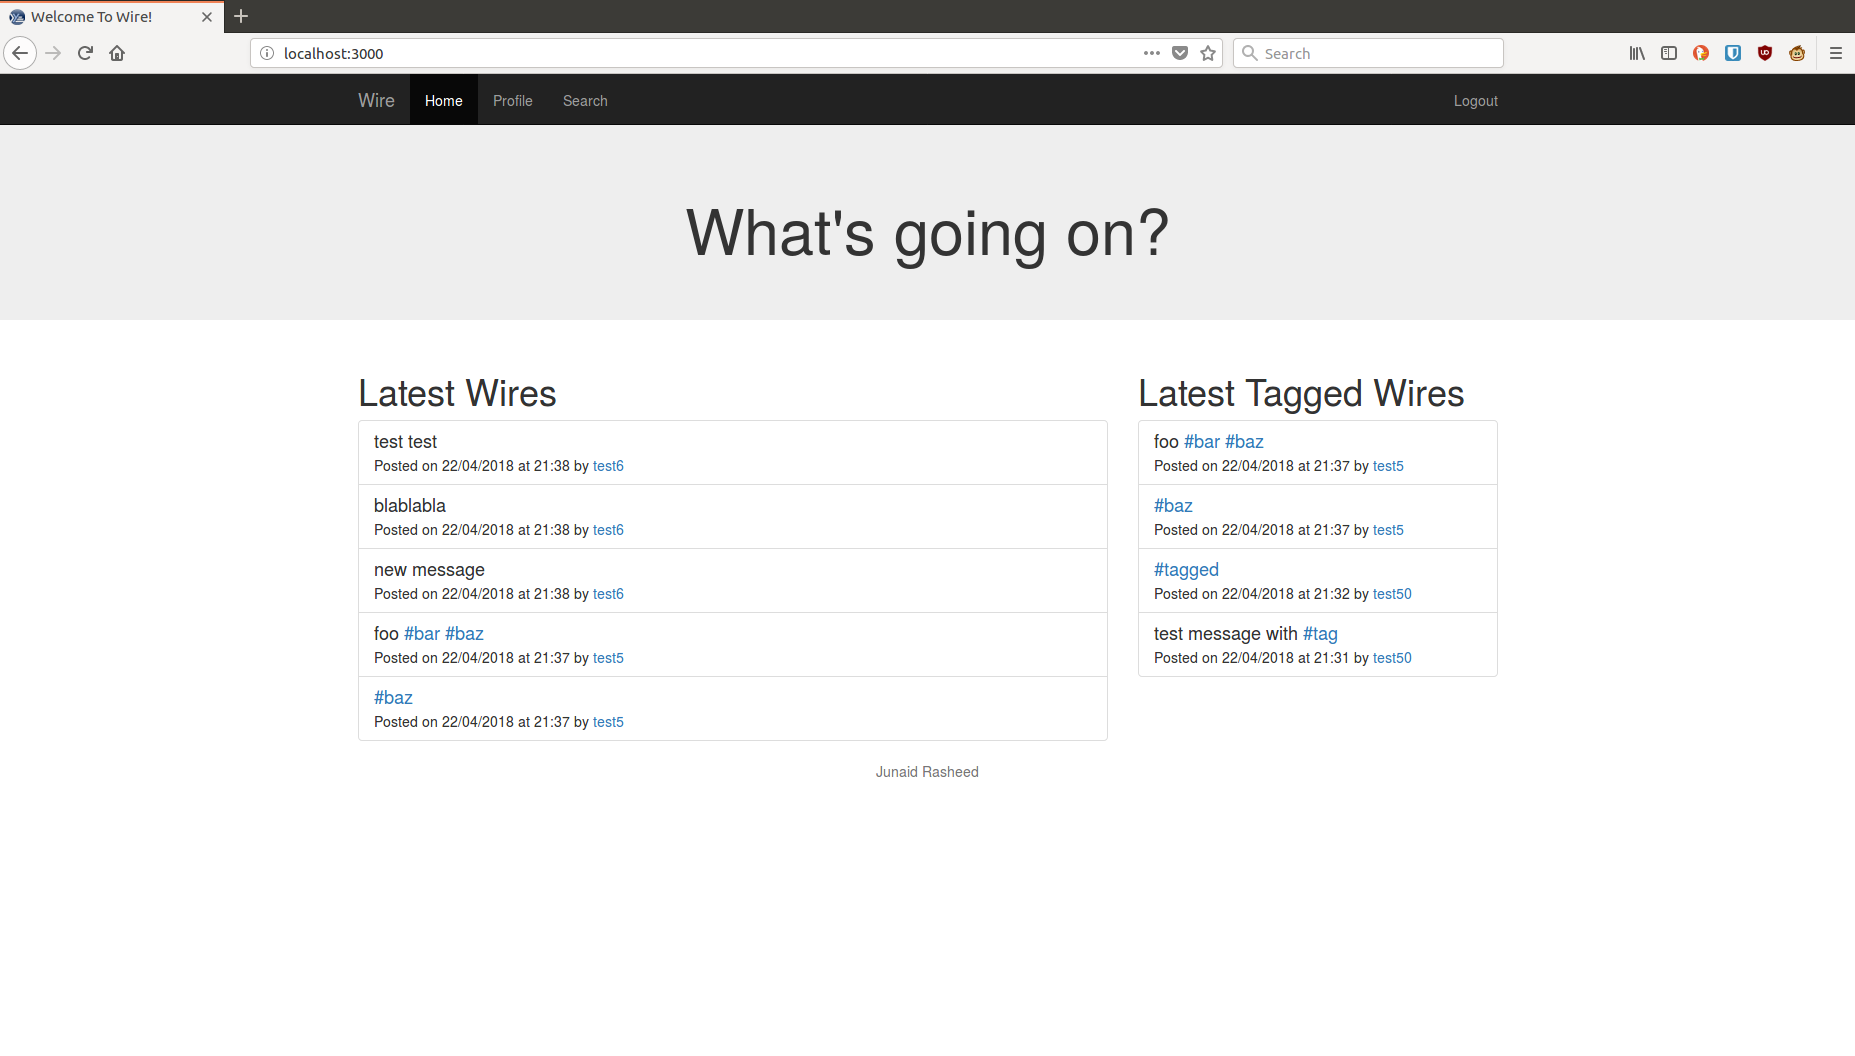
\includegraphics[width=0.7\textwidth]{final_report/pics/home.png}
    \caption{The home page}
    \label{fig:wireHome}
\end{figure}

The home page is the first page the user sees when they access the website.
The home page contains the latest messages posted by users on the website,
with a separate list for tagged messages. Messages that contain tags are links
that take the user to the search page. There is a navigation bar at the top of
the home page. This navigation bar is present on all pages. When a user is not
logged in, the navigation bar allows the user to access the login and signup pages.
Once logged in, the user can use the navigation bar to access their profile page
or to logout.

\subsection{Authentication}

\begin{figure}[htb]
    \centering
    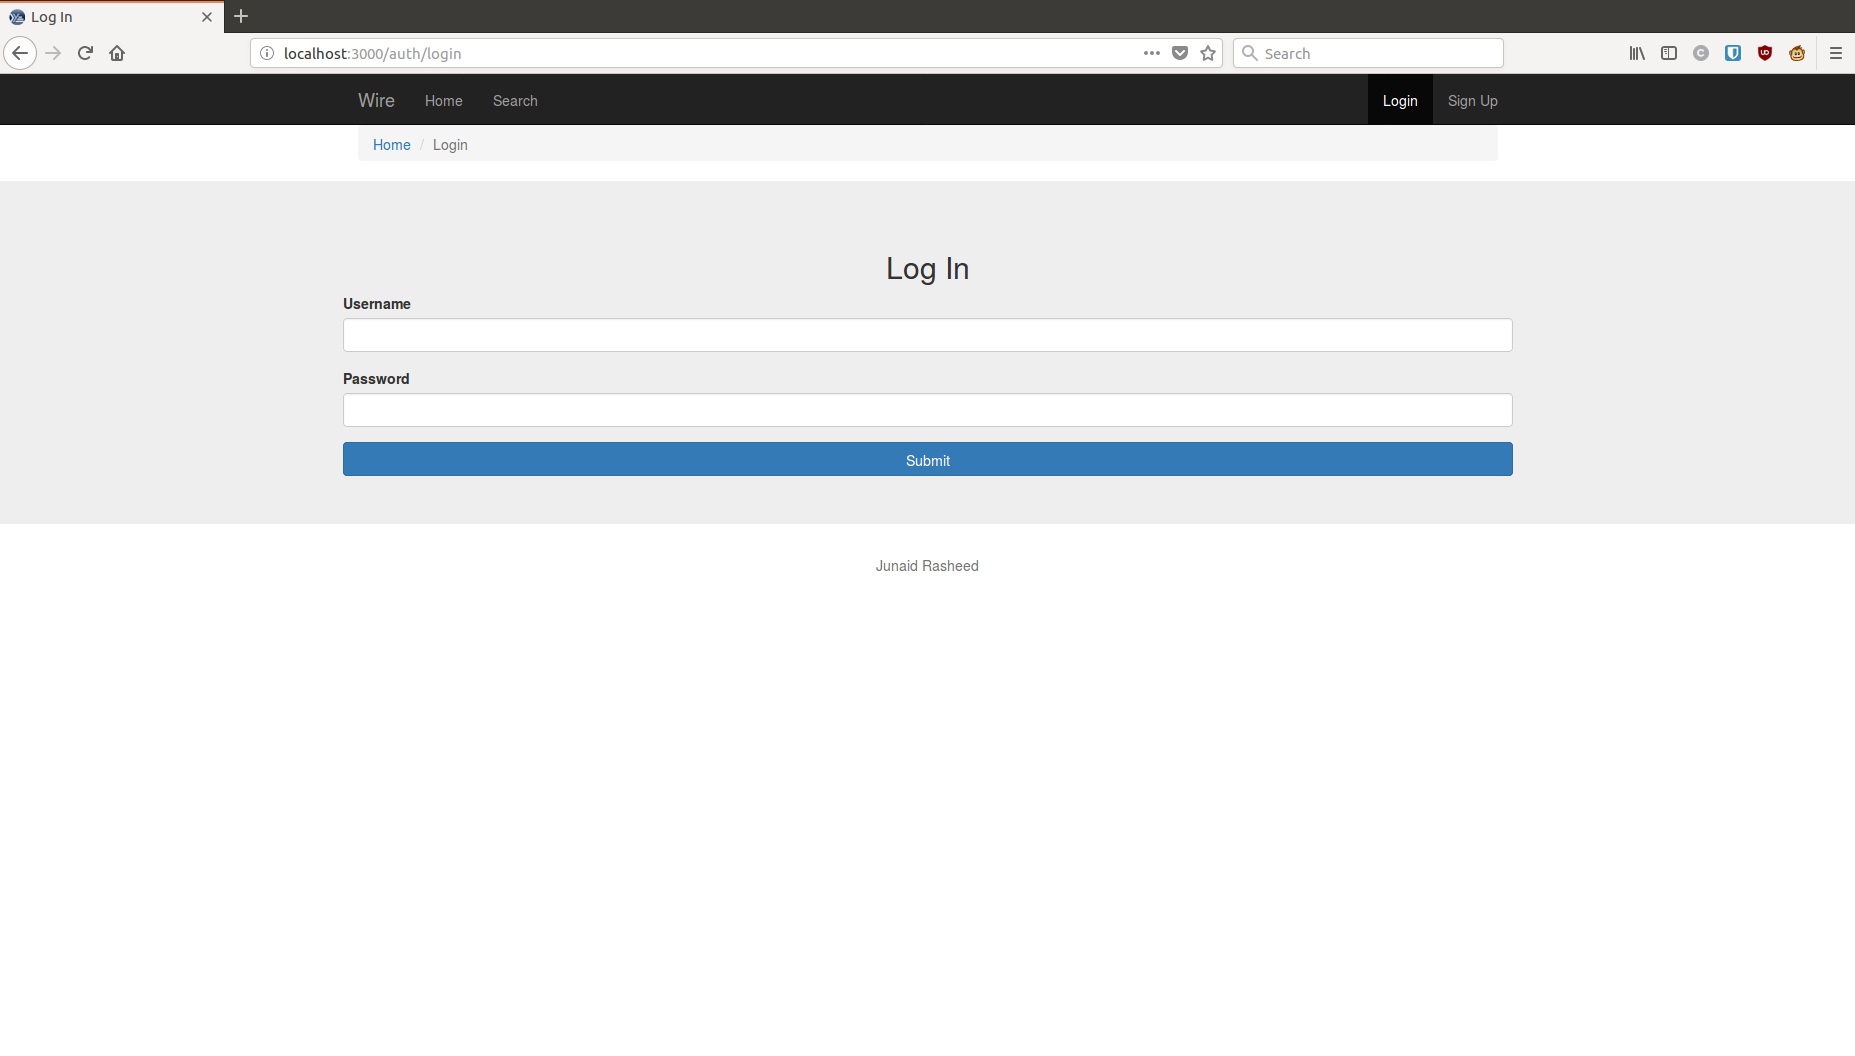
\includegraphics[width=0.7\textwidth]{final_report/pics/login.png}
    \caption{The login page}
    \label{fig:wireLogin}
\end{figure}

\begin{figure}[htb]
    \centering
    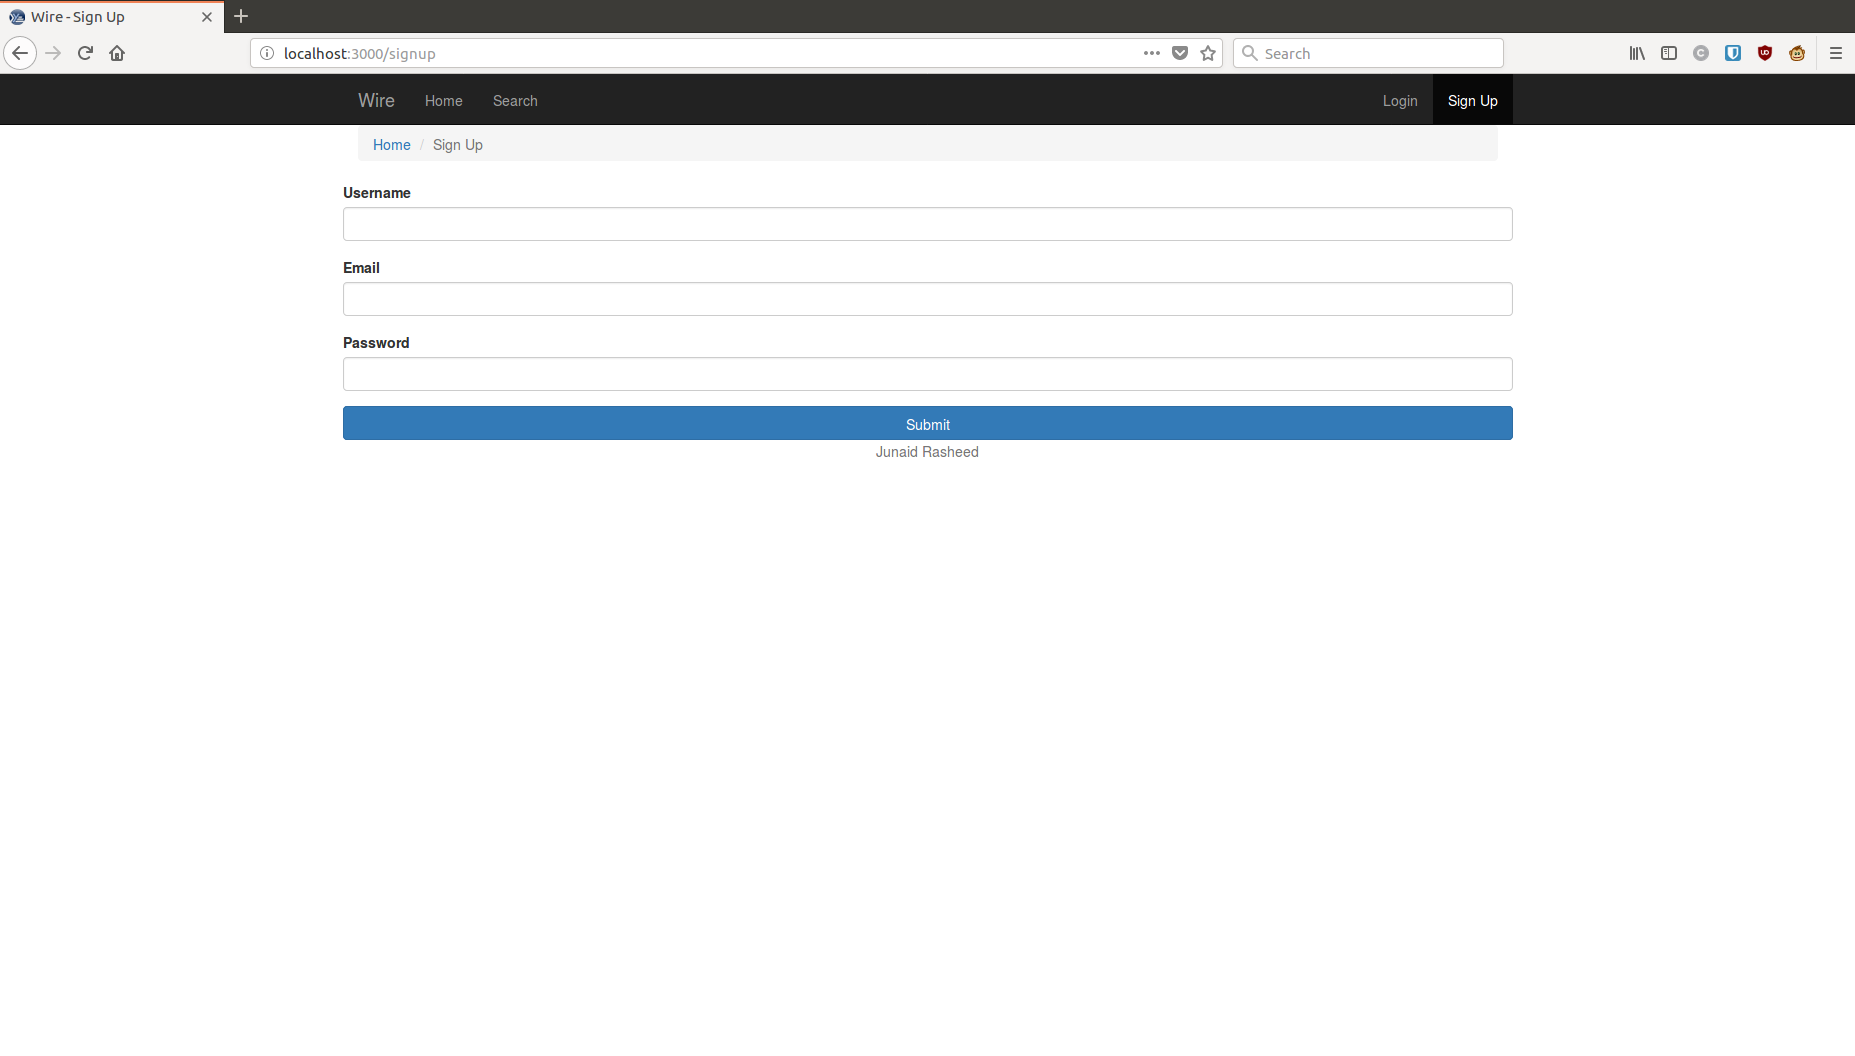
\includegraphics[width=0.7\textwidth]{final_report/pics/signup.png}
    \caption{The signup page}
    \label{fig:wireSignup}
\end{figure}

The authentication functionality of this website includes signing up and
logging in using a web page, and logging out using a button in the navigation
bar. In figure ~\ref{fig:wireSignup}, you can see that signing up requires
a username, e-mail, and password. The username and e-mail must be unique.
Users are shown a warning message if they try to sign up with details that
are already taken. Once a user signs up, their details are stored in the
database, with the password being hashed and salted to ensure that it is
stored safely.

When logging in, you only need to supply a username and password, as you can
see in figure ~\ref{fig:wireLogin}. This is because the username is a unique
identifier, we can use it to determine which user to log in as. When the username
and password is submitted, we look up the username in the database, encrypt the
password, and see if the encrypted password matches the one stored in the database. 
If there is a match, the user is authenticated and redirected to the home page. 
If there is an issue, the user is redirected back to the login page with an 
appropriate error messages.

Once the user is logged in, they can use the log out button which is present
on the top right of the navigation bar. Clicking this button immediately logs
the user out and they are redirected to the home page.

\subsection{User Profiles}

\begin{figure}[H]
    \centering
    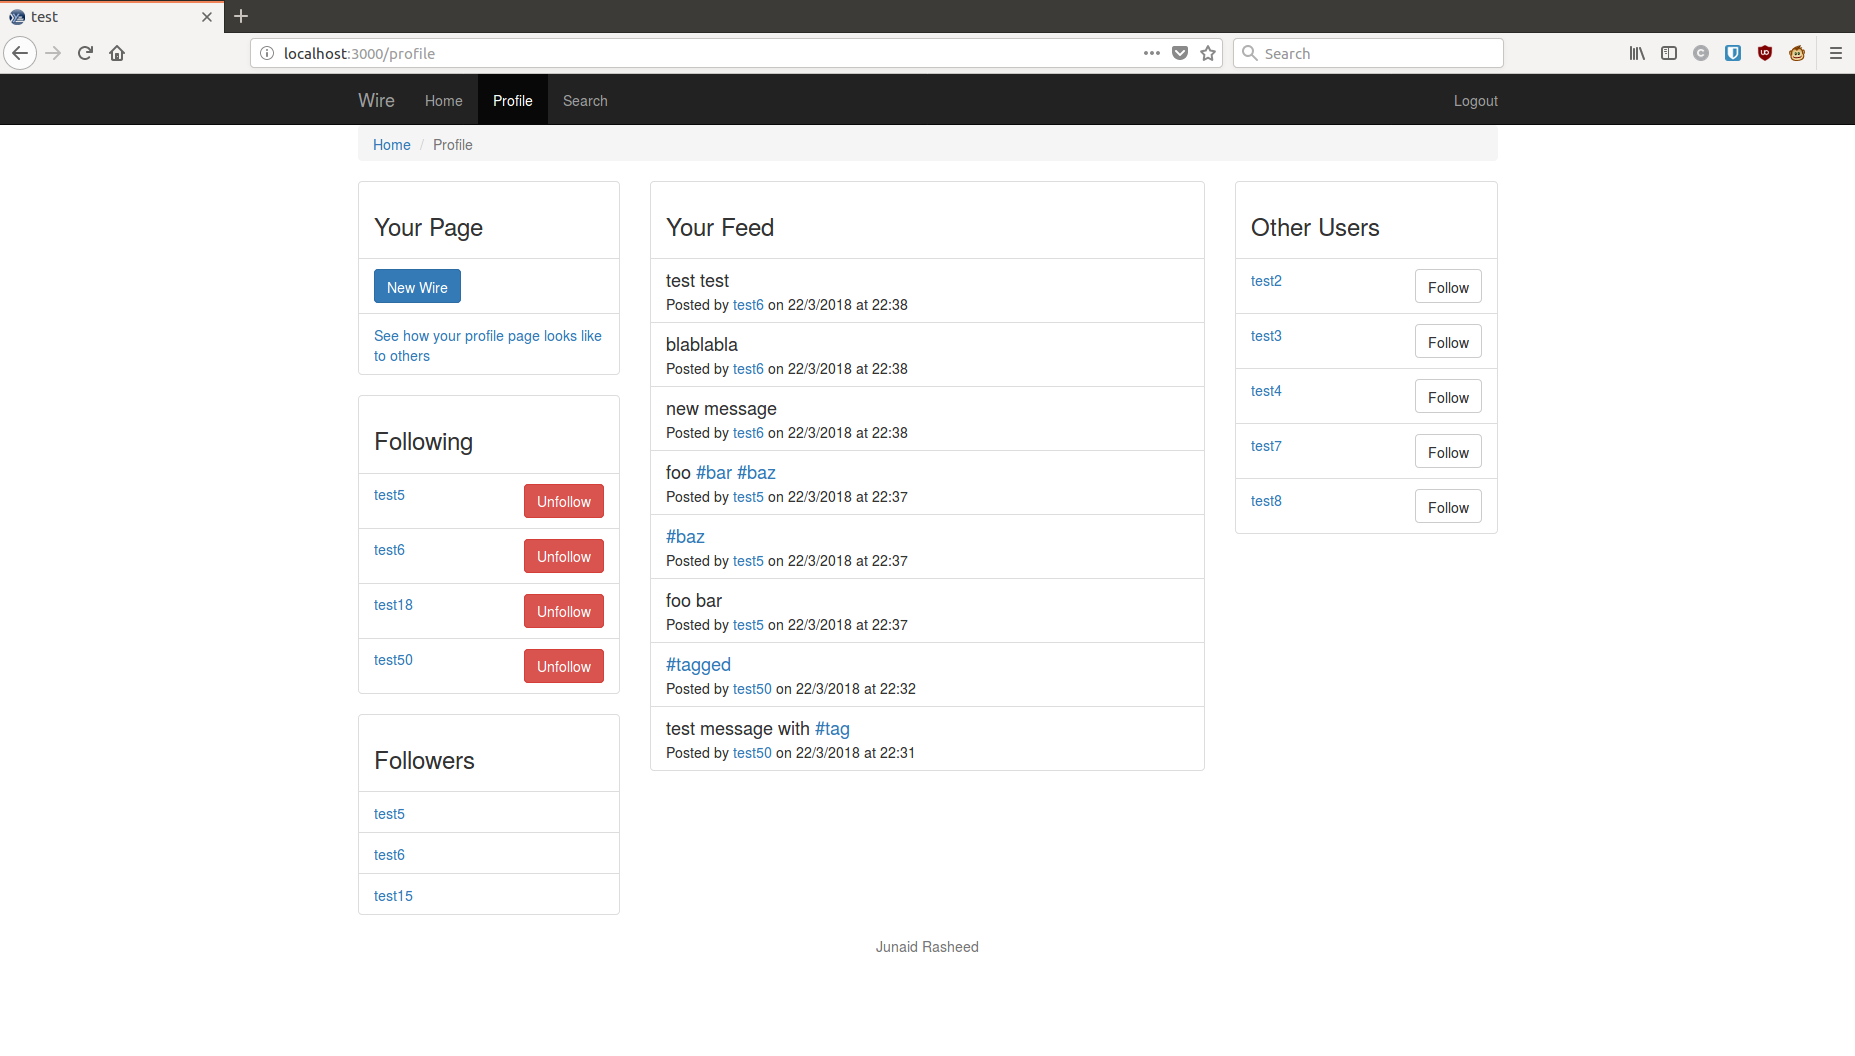
\includegraphics[width=0.7\textwidth]{final_report/pics/profile.png}
    \caption{The profile page for the current user}
    \label{fig:wireProfile}
\end{figure}

\begin{figure}[H]
    \centering
    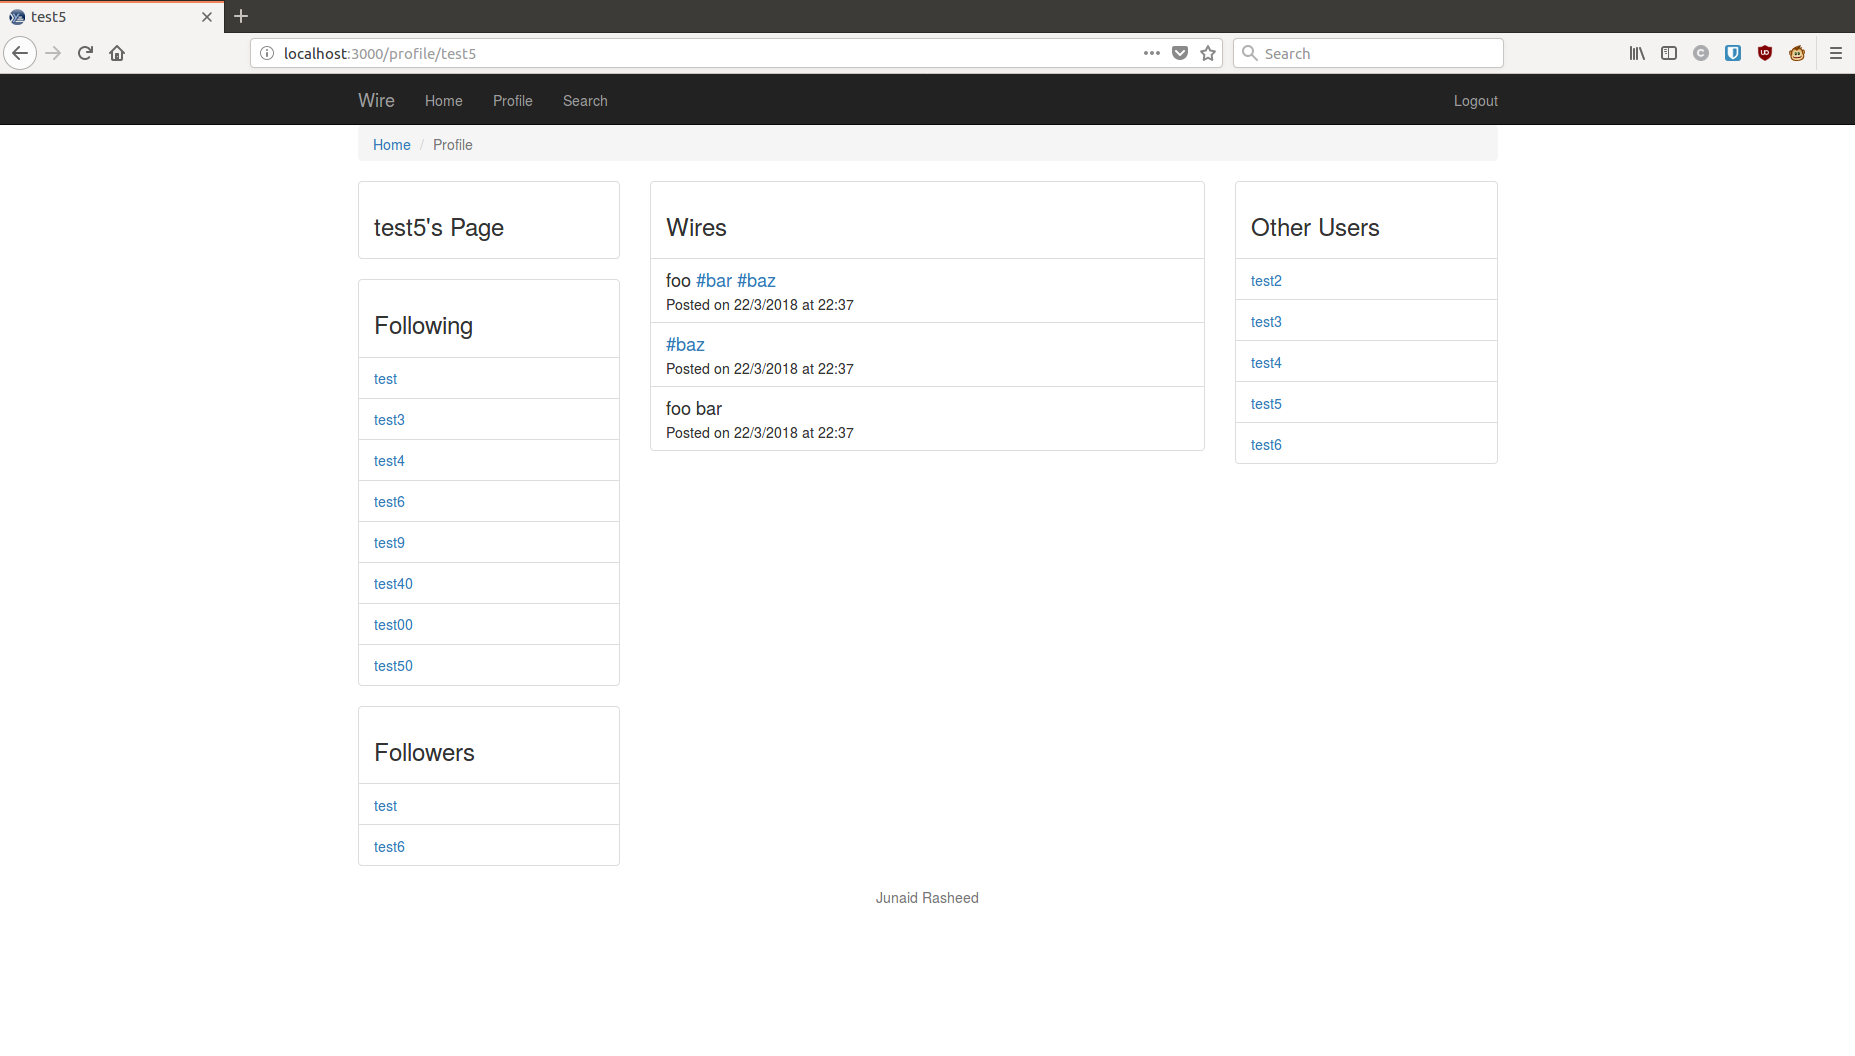
\includegraphics[width=0.7\textwidth]{final_report/pics/otherProfile.png}
    \caption{The profile page for other users}
    \label{fig:wireOtherProfile}
\end{figure}

\begin{figure}[H]
    \centering
    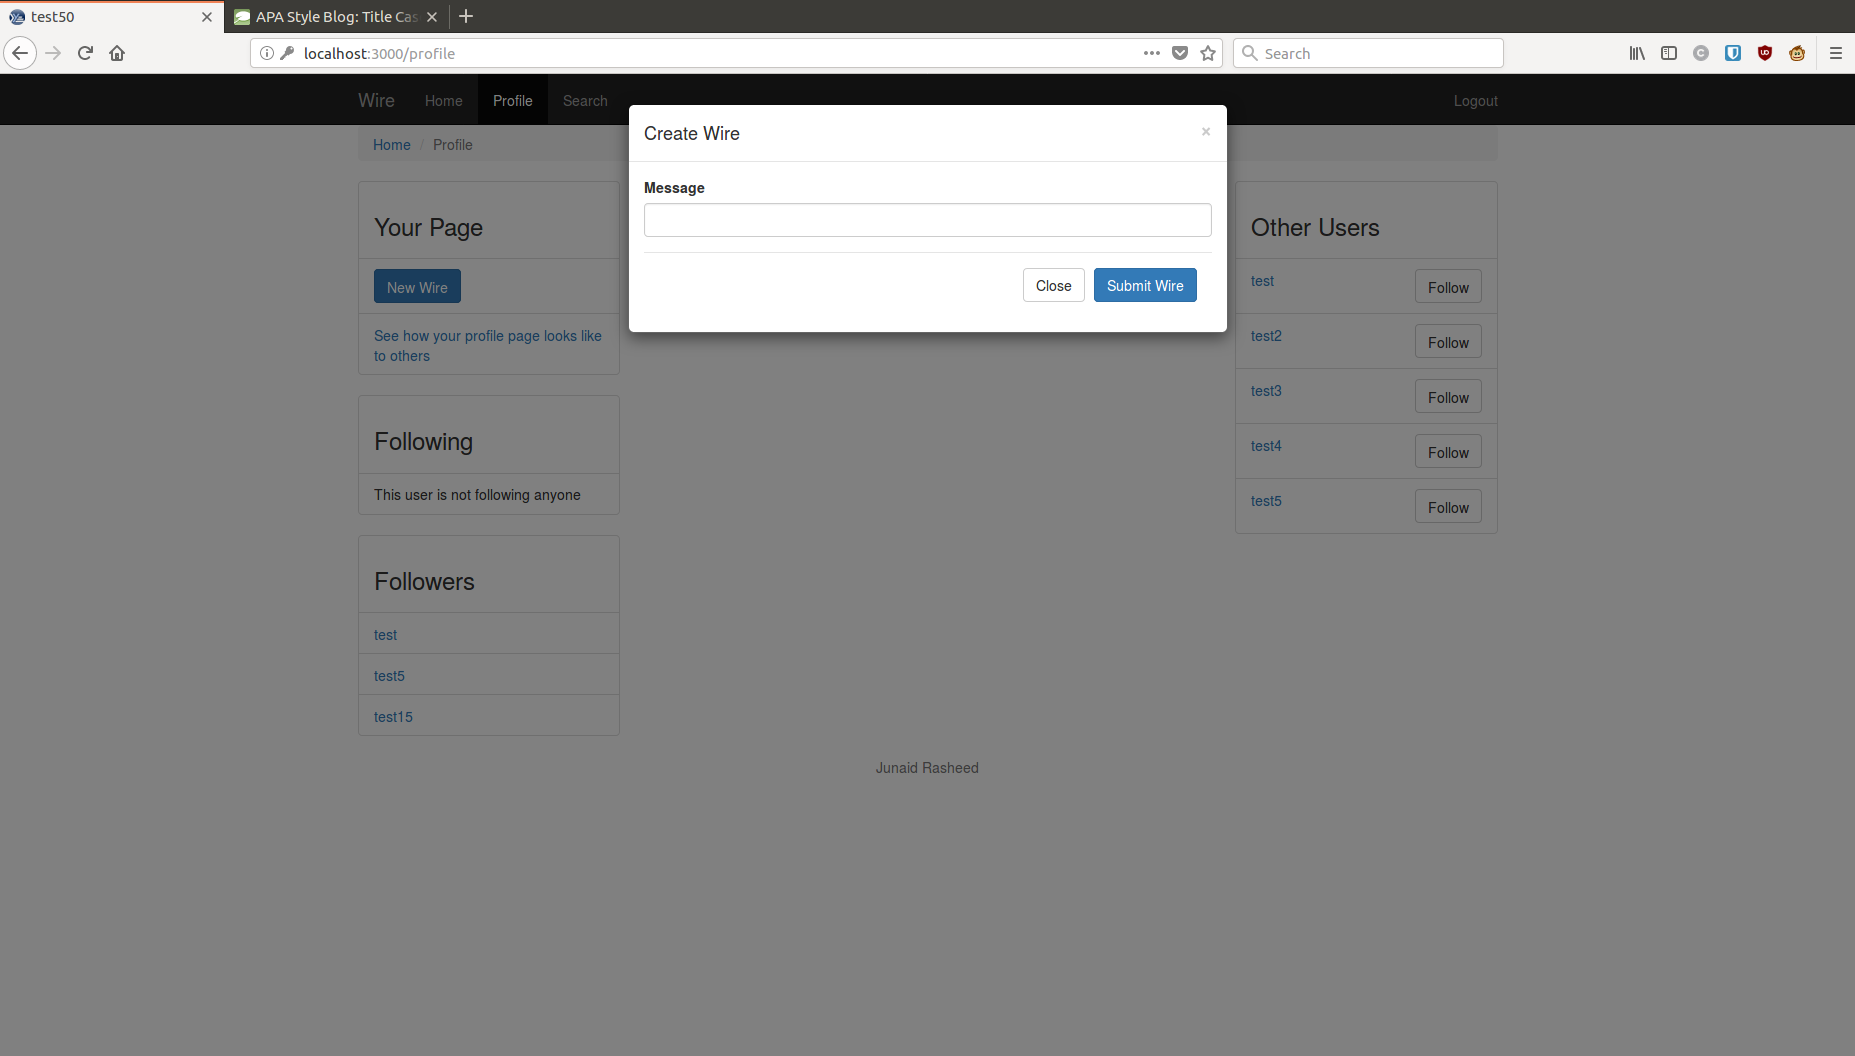
\includegraphics[width=0.7\textwidth]{final_report/pics/createWireForm.png}
    \caption{The create message form}
    \label{fig:wireCreateForm}
\end{figure}


The profile pages are probably the most complex with regards to logic in the
entire website. There are two different profile pages, one for the currently
logged in user which only they can see, and another for when someone is
viewing the profile page of another user.

Figure ~\ref{fig:wireProfile} is what a logged in user sees if they visit
their own profile page. On this page, they can see a list of messages posted
by users that they follow, see which users are following them, follow and
unfollow other users, and post their own messages. They can also post a
new message by clicking on the `New Wire' button. Clicking this button
displays a form which can be seen in figure ~\ref{fig:wireCreateForm}.

Figure ~\ref{fig:wireOtherProfile} is what the profile page looks like
when a user navigates to another person's profile page, or when they click
the `See how your profile page looks like to others' link on their own
profile page. This page shows the name of the person who owns the page,
the users they follow, other users that follow them, and messages that
they have posted.

One feature to note is that the messages and other user information on
the profile page is loaded in via AJAX. This ensures that the initial
page load is quick, following and unfollowing users does not necessitate
an entire page reload, and makes it easier to, if desired, add a feature
to automatically update the message area.

\subsection{The Search Page}

\begin{figure}[H]
    \centering
    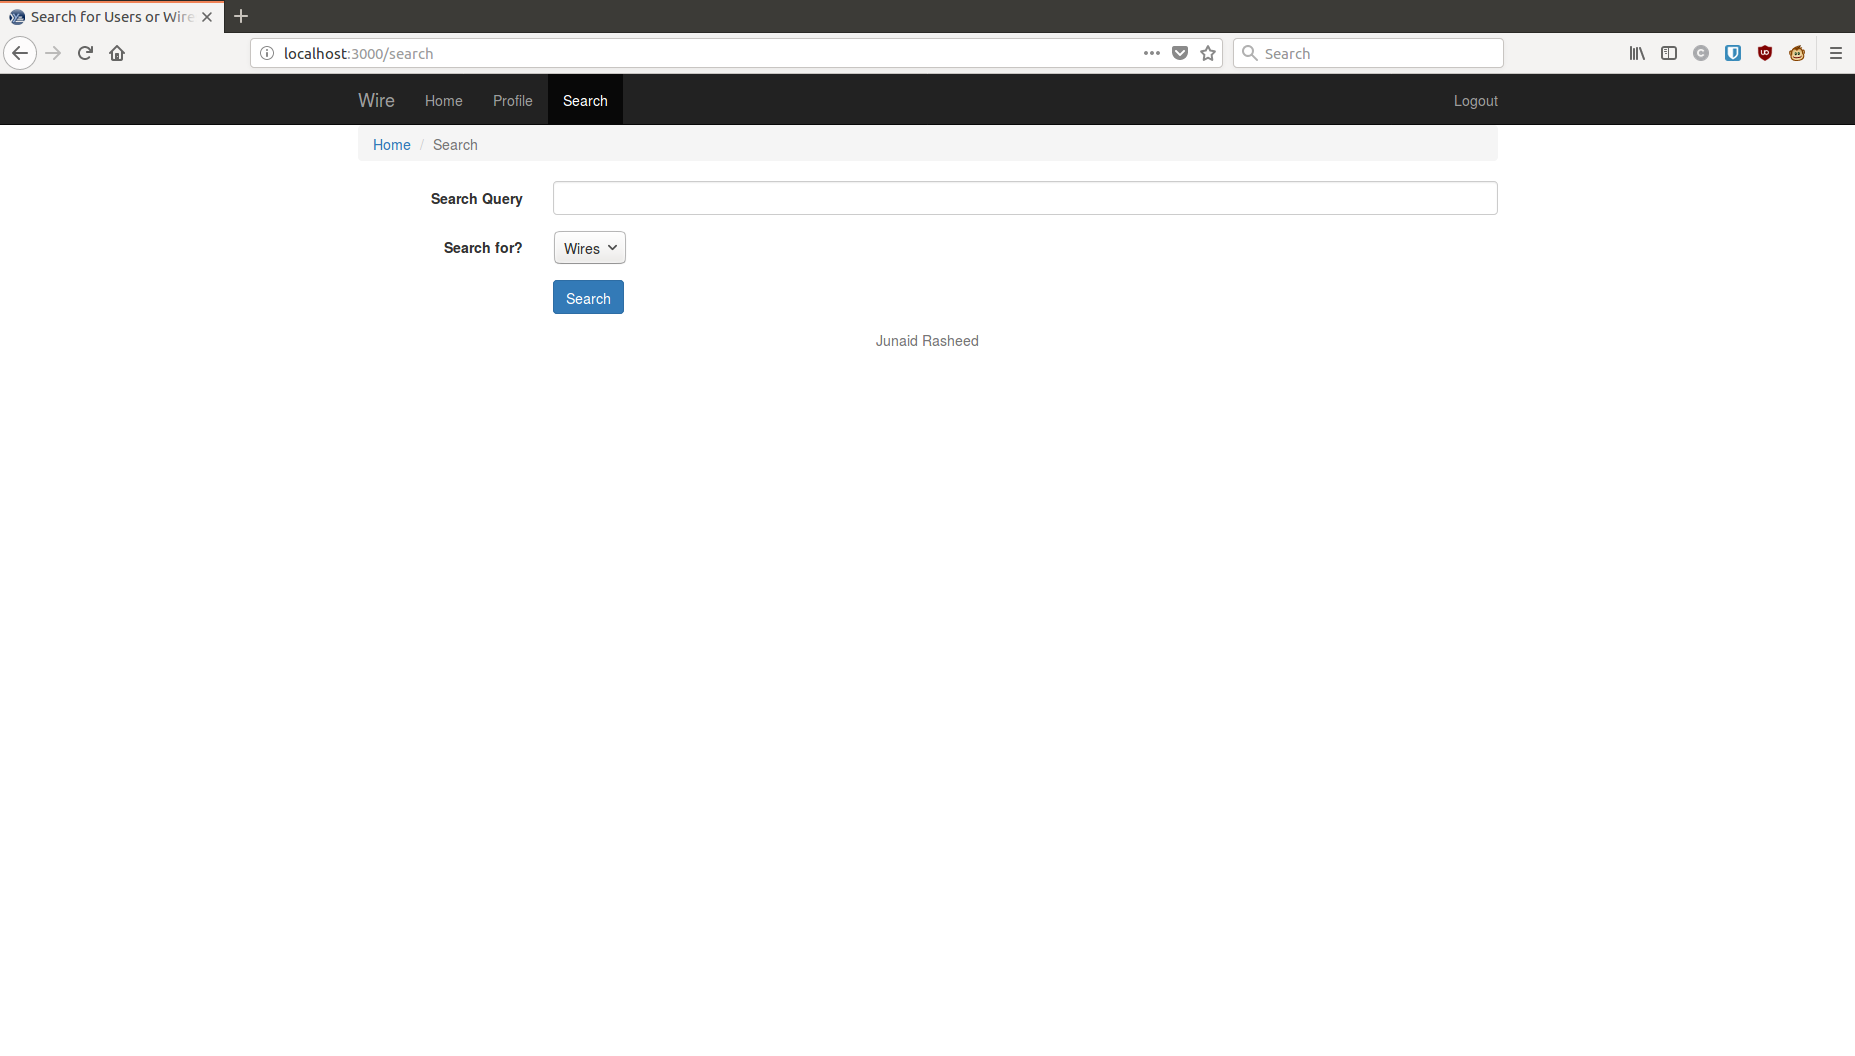
\includegraphics[width=0.7\textwidth]{final_report/pics/searchBase.png}
    \caption{The search page}
    \label{fig:wireSearch}
\end{figure}

\begin{figure}[H]
    \centering
    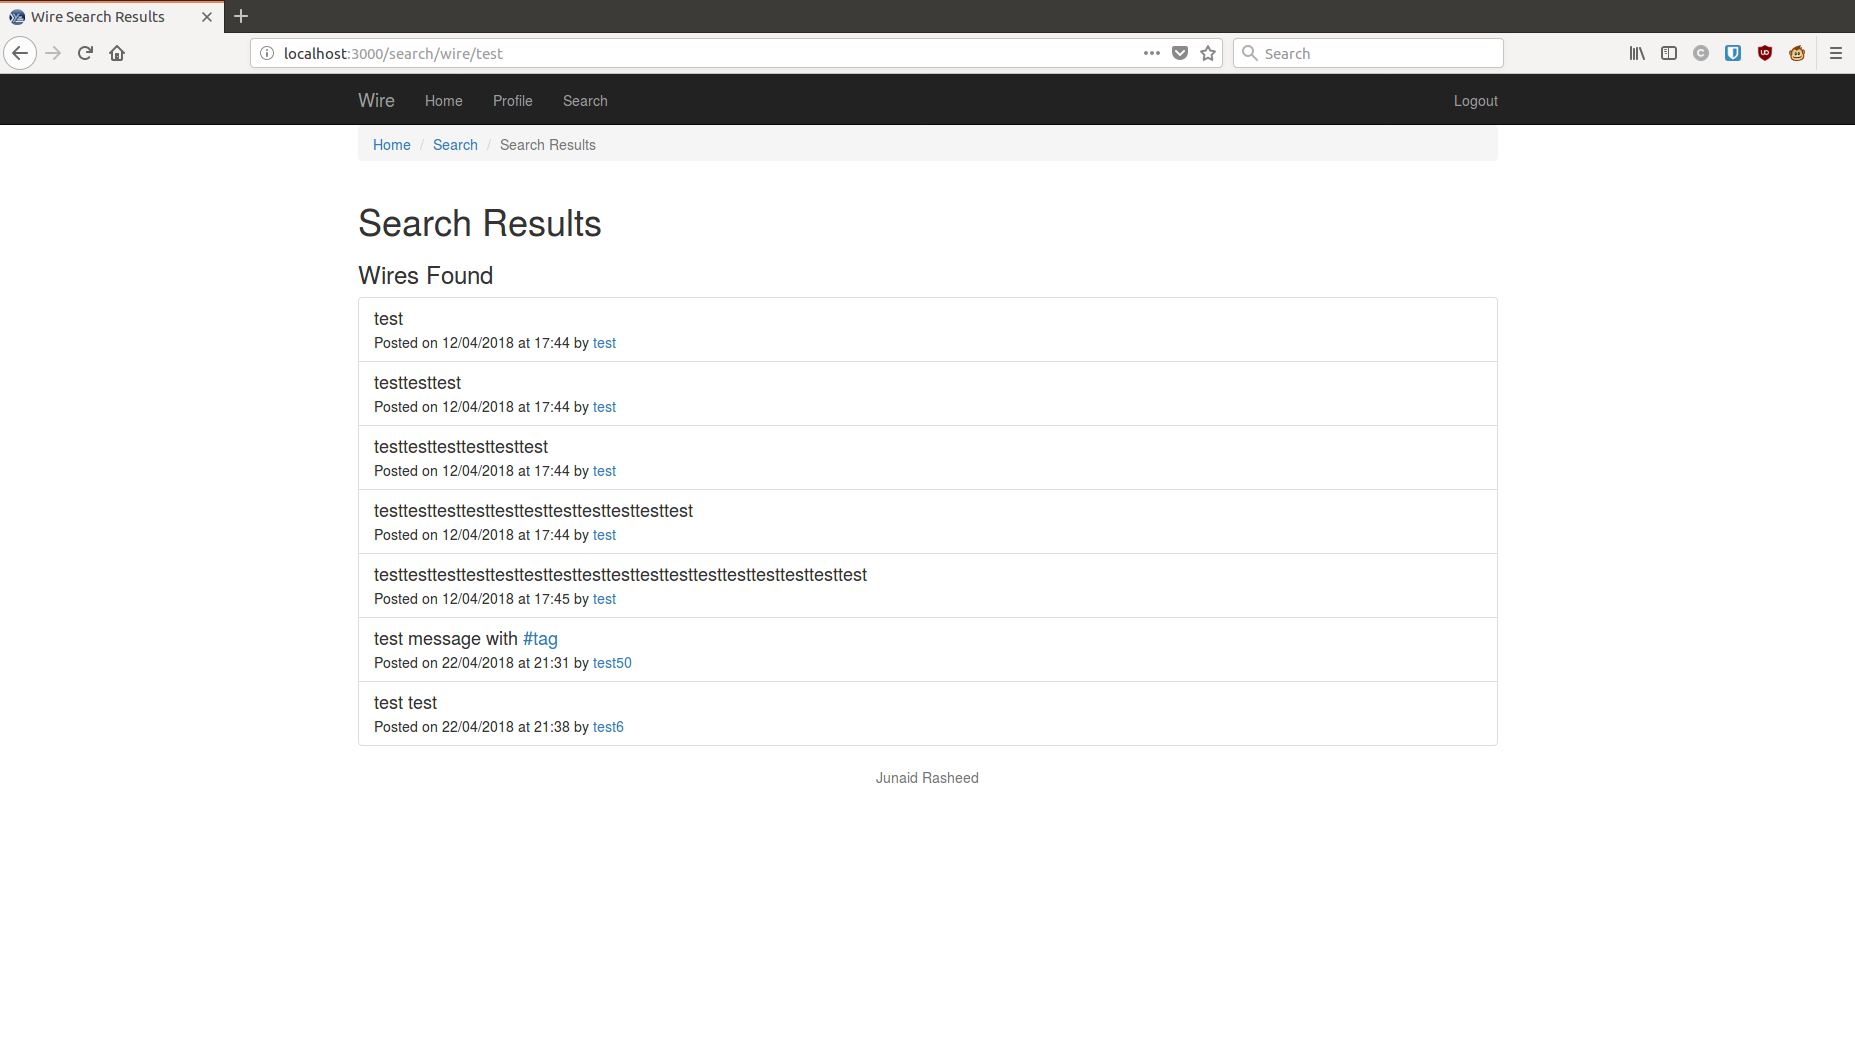
\includegraphics[width=0.7\textwidth]{final_report/pics/searchWire.png}
    \caption{The search results page for messages}
    \label{fig:wireSearchWire}
\end{figure}

\begin{figure}[H]
    \centering
    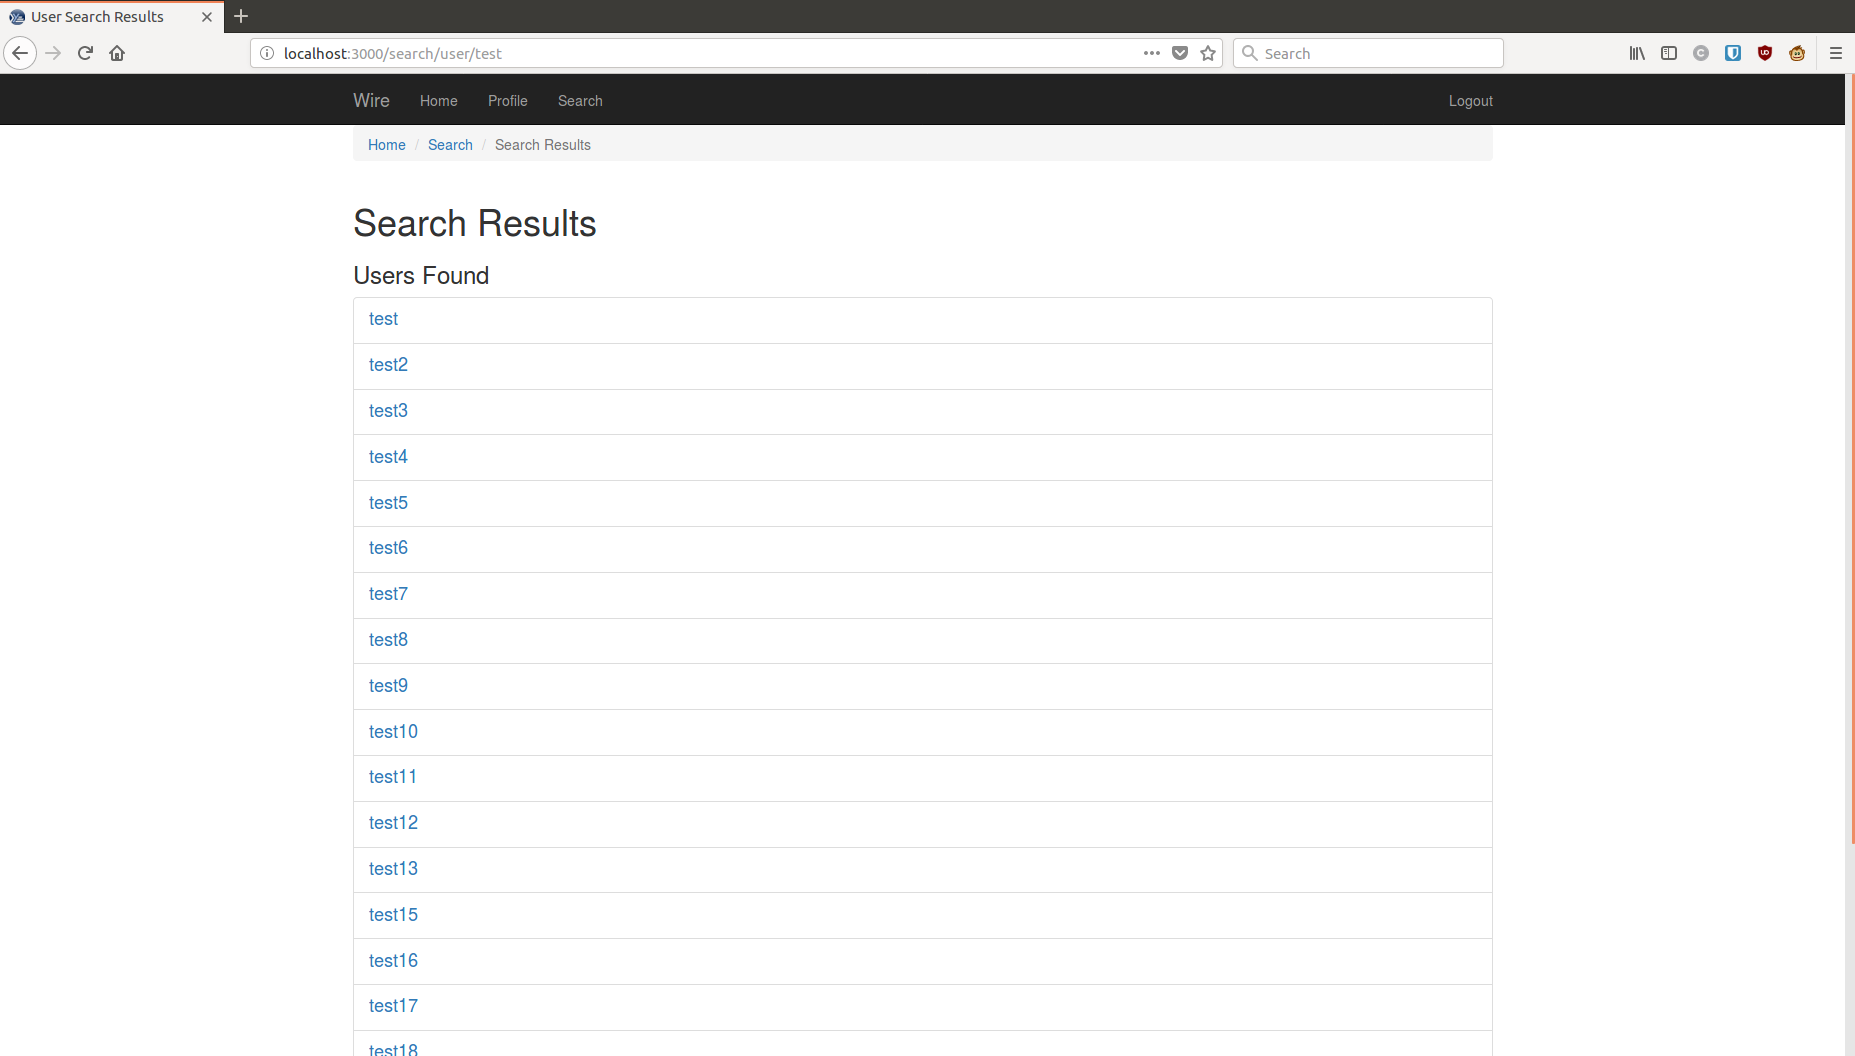
\includegraphics[width=0.7\textwidth]{final_report/pics/searchUser.png}
    \caption{The search results page for other users}
    \label{fig:wireSearchUser}
\end{figure}

Figure ~\ref{fig:wireSearch} is the page that the user is navigated to when they
click the search button in the navigation bar. In this page, they can type in
their search query and use the dropdown to specify whether they are searching
for users or messages. Once they submit their query, they are redirected to
the search results page, as seen in Figures ~\ref{fig:wireSearchUser} and
~\ref{fig:wireSearchWire}.

\section{The Yesod Implementation}

In this section, we will briefly discuss how the website was implemented in Yesod.
We will take a look at creating database entities, URL routing, handling requests,
creating templates, and writing tests.

\subsection{The Scaffold}
When creating a new Yesod site, it is recommended to use the scaffolding tool.
The scaffolding tool generates code that sets up the structure of your project. It
creates the files needed to connect to a database and launch a website. Sample code
is included for developers to see how the framework works. By running the scaffolding
tool, it is clear to the developer where source files, configuration settings, templates, and 
static files should be kept. \parencite[Scaffolding and the Site Template]{yesodBook}

The Yesod codebase used for this project was built on top of code generated by the
scaffolding tool using the yesod-postgres template, which tells the generated code
to be compatible with a PostgreSQL database.

\subsection{Defining Routes}

URL routes are available routes in an application and are specified in the 
`config/routes' file. In this file, you specify whether a request from a route is a
GET or POST request, the handler that deals with the request, and any parameters
that are part of the request. One of the features of Yesod is type safety in URLs,
so you can specify the actual type that a URL parameter should be. If the user
tries to navigate to a page with an invalid parameter, a 404 page will be shown.
An extract from the `config/routes' file can be seen in code block 
~\ref{code:yesodRoutes} below.

\lstset{language={}}

\begin{lstlisting}[caption={Yesod URL routes},label={code:yesodRoutes}]
    /profile MyProfileR GET POST
    /profile/#Text ProfileR GET
    
    /user UserGetAllR GET
    /user-not-following UserGetAllExcludingFollowingR GET
    /user/#Text UserGetAllExcludingUsernameR GET
    /user/id/#UserId UserGetIdR GET
    /users/*[UserId] UserGetIdsR GET
\end{lstlisting}

In code block ~\ref{code:yesodRoutes}, you can see that there
are two routes for the profile page. One, \texttt{/profile}, is for users
viewing their own profile page and the other, \texttt{/profile/\#Text}, are
for viewing the profile pages of the other users. The \texttt{\#Text} part
of the route specifies that there should be one parameter for this
route with the type \texttt{Text}. If multiple parameters are provided or a parameter
is not of the type \texttt{Text}, a 404 error is shown.

Further examples of URL parameters can be seen in the \texttt{user} routes. 
\texttt{/user/id/\#UserId} expects a user id as a parameter. If the specified
id is not found, a 404 page is shown. \texttt{/users/\*[UserId]} expects a list
of user ids, which would look like \texttt{/users/1/2/3/4/}.

\subsection{Database Entities}

Database entities are defined in the `config/model' file. In this file, you
give a name to the entity you want to create, the names and types of it's
fields, functions that the entity and it's fields should include, and
any fields that are unique, i.e. Cannot be shared with other entities.
Once an entity is added to this file, it is created in the database
when the codebase is compiled and helper functions are created that
can be used when programming. Code block ~\ref{code:yesodEntities} contains
the definition of the user entity extracted from the `config/models' file.

\begin{lstlisting}[caption={Yesod Database Entities},label={code:yesodEntities}]
    User json key
        username Text Eq
        email    Text Eq
        password Text
        UniqueUser username
        UniqueEmail email
        deriving Typeable Show
\end{lstlisting}

\subsection{Handlers}

Every URL route in the application points to a handler. Handlers are located in
the \texttt{src/handler} directory. They are used to perform any calculations or queries 
that need to be done and then respond to a request by rendering a template file, 
returning a JSON object, or by redirecting to another handler.

Code block ~\ref{code:yesodGetProfileR} is the handler used to respond to get requests
to display the profile page of the current user. The handler ensures the user is logged in,
loads the user's details, loads data on people being followed by the current user,
and then loads the template file. The parameters that are created and available
in the handler are also available in the template file.

\lstset{language={Haskell}}

\begin{lstlisting}[caption={GET request handler for current profile page},label={code:yesodGetProfileR}]
    -- Loads the 'My Profile' page for the currently logged in user. If someone
    -- who is not logged in attempts to access the page, a 404 error will be shown.
    getMyProfileR :: Handler Html
    getMyProfileR = do
        (Entity userId user) <- requireAuth
        let username = userUsername user
    
        -- Load messages posted by users followed by the current user
        follows <- runDB $ selectList [FollowFollowingId ==. userId] []
        let followIds = map (\(Entity _ (Follow followerId _)) -> followerId) follows
    
        (formWidget, formEnctype) <- generateFormPost $ messageForm userId
        defaultLayout $ do
            setTitle . toHtml $ userUsername user
            $(widgetFile "currentprofile")
\end{lstlisting}

You may have noticed the message form being generated in code block ~\ref{code:yesodGetProfileR}.
This form is defined in Haskell and the source code can be seen in code block ~\ref{code:yesodMessageForm}.
When defining the form, we give it a user id to specify the user creating a message, 
we tell the form that there is one input field that is required. Two hidden fields
are also included to ensure the form has all the data needed to create a message
when it is submitted.

\begin{lstlisting}[caption={The message form},label={code:yesodMessageForm}]
    messageForm :: UserId -> Form Message
    messageForm userId = renderBootstrap3 BootstrapBasicForm $ Message
        <$> areq textField (bfs ("Message" :: Text)) Nothing
        <*> pure userId
        <*> lift (liftIO getCurrentTime)
\end{lstlisting}

When the user submits the form, the post handler is ran, which can be seen in code block
~\ref{code:yesodPostProfileR}. In this handler, we use the function \texttt{runFormPost}
to check whether or not the form is valid. If the form is valid, the message is added
to the database and the profile page is reloaded with a success message. If there's an
issue with the form, the profile page is reloaded with an appropriate error message.

\begin{lstlisting}[caption={POST request handler for current profile page},label={code:yesodPostProfileR}]
    -- Create a new wire for the logged in user
    postMyProfileR :: Handler Html
    postMyProfileR = do
        (Entity userId _) <- requireAuth
        ((result, _), _) <- runFormPost $ messageForm userId
        case result of
            FormSuccess message -> do
                void $ runDB . insert $ message
                setSession "msgrendered" "true"
                setMessage $ renderSuccessMessage "Wire Sent"
                redirect MyProfileR
            FormFailure errors -> do
                let renderedMessages = map renderErrorMessage errors
                setSession "msgrendered" "true"
                setMessage $ toHtml renderedMessages
                redirect MyProfileR
            FormMissing -> do
                setSession "msgrendered" "true"
                setMessage $ renderErrorMessage "Form is missing"
                redirect MyProfileR
\end{lstlisting}

If a route contains a URL parameter, the handler must also have a parameter to store
the value of the given parameter. Code block ~\ref{code:yesodGetUserGetIdR} is the
source code for a handler that takes in a user id as a parameter. As you can see,
we do not have to check for the type of this parameter or whether it is not null.
We specified the type of the URL parameter in the routes file (code block ~\ref{code:yesodRoutes})
so Yesod will perform type checking for us, saving developers time from having
to manually deal with invalid types or values.

\begin{lstlisting}[caption={GET request handler for getting user data},label={code:yesodGetUserGetIdR}]
    -- | Takes in a user id and returns data on the user matching the given id.
    -- If no user is found, an empty JSON object is returned.
    getUserGetIdR :: UserId -> Handler Value
    getUserGetIdR userId = do
        users <- runDB $ selectList [UserId ==. userId] []
        let cleanUsers = map (\(Entity uid (User uname _ _)) -> (object ["id" .= uid, "username" .= uname])) users
        returnJson cleanUsers
\end{lstlisting}

\subsection{Templates}

The templates used in Yesod are called Shakespearean templates. Shakespearean templates
allow you to write type-safe templates that are compiled, helping prevent runtime errors.
The syntax for Shakespearean templates are similar to the languages they are based on,
with minor changes to the syntax used in the templates. For example, the HTML template language, Hamlet,
uses indentation rather than opening and closing tags to denote nesting. Within these
templates, you can use Haskell variables, create type-safe routes, and implement conditional
and looping logic. \parencite[Shakespearean Templates]{yesodBook}

When a template file is loaded in a handler, the file is actually included inside
a default file. The default file contains content that is common to all pages. This
ensures that code does not need to be repeated, reducing the chance of mistakes and
making it easier to change the layout of the whole site.

A simple template file can be seen in code block ~\ref{code:yesodSearchHamlet}. In this
block, you can see how indentation is used to determine nesting. Variable interpolation
is done using \texttt{\#\{variableName\}}. You can see the form is being loaded using
the \texttt{\string^\{widgetName\}}, which renders the given widget onto the page. Type safe
URLs are loaded using \texttt{\string@\{routeName optionalParameters\}}.

\begin{lstlisting}[caption={Template file for the search page},label={code:yesodSearchHamlet}]
    <main>
        <div .container>
            <div .row>
                <div .col-sm-12>
                    <form #search-form .inline .form-horizontal role=form method=post action=@{SearchR} enctype=#{formEnctype}>
                        ^{formWidget}

\end{lstlisting}

\subsection{Tests}
The Yesod test suite allows you to create BDD-style tests. When creating a test,
you specify what it should do, create any database entities you need, make a
request to a handler, and examine the response to see if the data you received
is correct. Code block ~\ref{code:yesodGetProfileTest} is an actual test
from the website. The test creates and logs in as a new user, loads
the profile page, and ensures that the resulting HTML contains the text that
it should contain. Yesod gives you the ability to use CSS selectors when checking
the HTML page given by a response, allowing you to be very specific.

\begin{lstlisting}[caption={Test the profile page},label={code:yesodGetProfileTest}]
    it "asserts that the current profile page looks right" $ do
        foo <- createUser "foo" "foo@bar.com" "foo"
        authenticateAs foo

        get MyProfileR
        htmlAnyContain "h3" "Your Page"
        htmlAnyContain "h3" "Your Feed"
        htmlAnyContain "h3" "Followers"
        htmlAnyContain "h3" "Following"
        htmlAnyContain "h3" "Other Users"
\end{lstlisting}

The testing suite also has the ability to check if a JSON response contains the
data that we expect. However, you do not have the same helper functions available
to you when compared to checking HTML responses. When checking JSON response, you
must examine the body of the response itself. You cannot check if a JSON key has
a given value. See code block ~\ref{code:yesodGetAllUsers} below.

\begin{lstlisting}[caption={Checking a JSON response},label={code:yesodGetAllUsers}]
    it "asserts all users are returned when not authenticated" $ do
        _ <- createUser "foo" "foo@bar.com" "foo"
        _ <- createUser "bar" "bar@bar.com" "foo"
        _ <- createUser "baz" "baz@bar.com" "foo"

        get UserGetAllR

        bodyContains "username"
        bodyContains "id"
        bodyNotContains "email"
        bodyNotContains "password"
        bodyContains "foo"
        bodyContains "bar"
        bodyContains "baz"
\end{lstlisting}
\section{The Django Implementation}
Now, we will discuss how the Django site was implemented. We will go through Django apps,
routes, entities, views, templates, and tests.

\subsection{Creating a Project}
All Django sites require a Django project. A project is
a directory that contains all the settings needed for a Django website. This includes
database settings, the apps being used, application settings, and Django-specific
settings. To create the project, the \texttt{django-admin} tool was used. This tool
generates the code needed to connect to a database and start a Django site. \parencite{djangoIntroDocs}

\subsection{Creating Apps}

The code used for the actual web application resides in two Django apps, \texttt{base} and
\texttt{wire\_profile}. In Django, an app is a web application that can be a part of a project.
These apps contain the URL routes used in the application, database entities, views
that respond to requests, templates, and tests. The \texttt{manage.py} tool provided
by Django was used to create apps. This tool creates a directory with a specified name
and a layout of files and directories that is preferred for Django apps. \parencite{djangoIntroDocs}

\subsection{Routes}

Django routes are specified in the \texttt{urls.py} file within an app. The routes
specify a URL path, a view that responds to requests from the given path, and a name
that is used to refer to a route within code. Django routes can contain URL parameters,
like Yesod. The valid values for these parameters can be defined using regular expressions
or a few built in types like \texttt{string} or \texttt{int}. To denote a list of parameters,
\texttt{path} can be used. An example of Django routes can be seen in code block ~\ref{code:djangoRoutes}.

\lstset{language={Python}}

\begin{lstlisting}[caption={An extract of Django routes},label={code:djangoRoutes}]
    path('following/<path:username>', views.get_following, name='get_following'),
    path('users/<path:user_ids>', views.get_user_ids, name='get_user_ids'),
    path('user/id/<int:user_id>', views.get_user_id, name='get_user_id'),
    path('search', SearchView.as_view(), name='search'),
\end{lstlisting}

\subsection{Database Entities}

Database entities are defined as models in the \texttt{models.py} file within an app.
In this file, the name of a database entity is mapped to a class in the file. The variables inside
this class are used to determine the names and types of entity's fields. You can see
an example of a Django model in ~\ref{code:djangoEntities}. When an entity is created 
or modified, Django migrations must be created and then ran using the \texttt{manage.py} tool. 
Migrations are used by Django to ensure changes you make to models are executed in 
the database schema. \parencite{djangoMigrations}.

\begin{lstlisting}[caption={The user entity in Django},label={code:djangoEntities}]
    class Message(models.Model):
    message_text = models.CharField(max_length=280)
    created = models.DateTimeField('created')
    user = models.ForeignKey(User, on_delete=models.CASCADE)

    def __str__(self):
        return self.message_text
\end{lstlisting}

\subsection{Views}

Views in Django are similar to Handlers in Yesod, they are used to determine
a response for a given request. There are two main types of views that you can
create in Django, class-based views and function-based views. The Django website
produced contains a mixture of class-based and function-based views.

Code block ~\ref{code:djangoCurrentProfileView} is a class-based view used to
render the profile page for the current user. In this view, we check if the
user is authenticated and then render the profile page for the authenticated
user. If the user is not authenticated, we redirect them to the home page and
show an error message.

\begin{lstlisting}[caption={Class-based current profile view},label={code:djangoCurrentProfileView}]
    class CurrentProfileView(TemplateView):
    template_name = "wire_profile/current_profile.html"

    def get(self, request, *args, **kwargs):
        """
        Get the current profile if the user is logged in.

        :param request: The current request
        :param args: sent to parent method
        :param kwargs: sent to parent method
        :return: Either redirect to the search page or render the profile page
        """
        if request.user.is_authenticated:
            context = self.get_context_data(**kwargs)
            form = NewWireForm()
            context['form'] = form
            context['user'] = request.user
            return self.render_to_response(context)
        else:
            messages.error(request, 'You must log in to view your profile page', extra_tags='danger')
            return HttpResponseRedirect(reverse('base:home'))
\end{lstlisting}

In the current profile view, we load a Django form for a user to create a message,
just like we do in Yesod. This form is located in the \texttt{forms.py} file. The
form, as seen in code block ~\ref{code:djangoMessageForm}, is a class where variables map
to input names. The Django form only requires one field, the message. No hidden
fields are used to determine the user that created a message, this is done in
the view itself.

\begin{lstlisting}[caption={Django message form},label={code:djangoMessageForm}]
    class NewWireForm(forms.Form):
        message = forms.CharField(widget=forms.Textarea(attrs={'rows': '3', 'cols': '40'}), label='Message', max_length=280)
\end{lstlisting}

When the form is submitted, a post request is sent to the function-based view
seen in code block ~\ref{code:djangoCreateMessageView}. In this view, the following
conditions are checked: whether or not the request type is POST, the validity of the
form, and whether or not the user is authenticated. If these conditions are true,
the message is created and saved to the database. If not, an appropriate error
message is rendered.

\begin{lstlisting}[caption={Function-based create message view},label={code:djangoCreateMessageView}]
    def create_message(request):
        """
        Create a message for the logged in user

        :param request: The request sent by the user
        :return: Display the profile page with a relevant message
        """
        if request.method == 'POST':
            form = NewWireForm(request.POST)
            if form.is_valid():
                if request.user.is_authenticated:
                    message = form.cleaned_data['message']
                    try:
                        Message.objects.create(message_text=message, created=timezone.now(), user=request.user)
                        messages.success(request, 'Message created successfully', extra_tags='success')
                        return HttpResponseRedirect(reverse('wire_profile:current_profile'))
                    except DatabaseError:
                        messages.error(request, 'Error creating message, please contact support', extra_tags='danger')
                        return HttpResponseRedirect(reverse('wire_profile:current_profile'))
                # ... each else condition renders an appropriate error message
\end{lstlisting}

The method to retrieve URL parameters in Django differ depending on the type
of view you use. For class-based views, URL parameter values are retrieved using
the \texttt{kwargs} variable available in all class-based views, as seen in
code block ~\ref{code:djangoSearchMessage}. For function-based views, a
parameter is added to the function itself, as seen in code block ~\ref{code:djangoGetUserIds}. 

\begin{lstlisting}[caption={Function-based view for returning user data},label={code:djangoGetUserIds}]
    def get_user_ids(request, user_ids):
        """
        Get the users with the given IDs in JSON format

        :param request: The request that called this function
        :param user_ids: The user ids to get the users for
        :return: list of users in JSON format
        """
        user_ids_list = filter(bool, user_ids.split('/'))
        user_ids_list = list(map(int, user_ids_list))
        % users = User.objects.filter(pk__in=user_ids_list).values('username')
        return JsonResponse(list(users), safe=False)
\end{lstlisting}

\begin{lstlisting}[caption={Class-based view to search for a given message},label={code:djangoSearchMessage}]
    class SearchMessageView(TemplateView):
        template_name = 'wire_profile/search_message.html'

        def get(self, request, *args, **kwargs):
            """
            Render the matching messages for a search message query

            :param request: The current request
            :param args: sent to parent method
            :param kwargs: sent to parent method
            :return: Render the search message results page
            """
            query = self.kwargs['query']
            search_results = Message.objects.filter(message_text__icontains=query).all()
            context = self.get_context_data(**kwargs)
            context['search_results'] = search_results
            return self.render_to_response(context)
\end{lstlisting}

\subsection{Templates}
The Django template language can be used in any HTML, CSS, and JavaScript
file. The Django template language can be used to perform variable interpolation,
conditional checks, loops, and creating default blocks of code that can be reused
in other templates. Rendering these files executes the the template logic that the
file contains. \parencite{djangoTemplates}

\begin{lstlisting}[caption={Template file for the search page},label={code:djangoSearchTemplate}]
    

    
    
    
    
    
        {{ block.super }}
        
    
    
    
        Search
    
    
    
    <main>
        <div class="container">
            <div class="row">
                <div class="col-sm-12">
                    <form id="search-form" class="inline form-horizontal" role=form method=post action="/search">
                        
                        
                    </form>
                </div>
            </div>
        </div>
    </main>
    
\end{lstlisting}

Code block ~\ref{code:djangoSearchTemplate} contains the source code for the
template file used to render the search page. In this file, a base template
is loaded, which is a full HTML page with the content divided up
into a number of blocks. These blocks are then overridden in the search template
to define breadcrumbs, set the page title, and write the markup for the main
content of the page. Laying out template files like this eliminates repetitive
code and keeps the Django template files similar to their Yesod counterparts,
reducing the need to design different templates in both frameworks.

\subsection{Tests}

Django tests are contained in the \texttt{tests.py} file within an app. Tests
are functions within a class. The process for testing in Django is similar to
Yesod: we create any needed database entities at the beginning of a test,
make a request, and check to see if the response is what we expect. Code
block ~\ref{code:djangoCurrentProfileTest} is a test where a user account
is created, logged in, and then the profile page for the user is loaded.
Django does not have the functionality available in Yesod that allows you
to test the content of a HTML page using CSS selectors, so instead, we test
that the correct template is being loaded with the expected template variables.

\begin{lstlisting}[caption={Django current profile test},label={code:djangoCurrentProfileTest}]
    class CurrentProfileViewTest(TestCase):
        # Other tests...
        def test_current_profile_page_for_logged_in_users(self):
            user = User.objects.create_user('testfoo', 'test@test.com', 'test')
            self.client.post(reverse('base:verify'), {'username': user.username, 'password': 'test'})
            response = self.client.get(reverse('wire_profile:current_profile'))

            self.assertEqual(response.status_code, 200)
            self.assertEqual(response.context['user'], user)
            self.assertIsInstance(response.context['form'], NewWireForm)
            self.assertTemplateUsed(response, 'wire_profile/current_profile.html')
\end{lstlisting}

In Django, we can still examine the content of a response, as seen in code block ~\ref{code:djangoCheckJsonResponse}.
In this block, we make a JSON request decode the response, ensuring that the response
content contains the expected data.

\begin{lstlisting}[caption={Django checking a JSON response test},label={code:djangoCheckJsonResponse}]
    class GetUserIdsTest(TestCase):
        # Other tests...
        def test_get_user_ids_one_user(self):
            user = User.objects.create_user('foo', 'test@test.com', 'test')
            user2 = User.objects.create_user('bar', 'bar@test.com', 'test')
            user3 = User.objects.create_user('baz', 'baz@test.com', 'test')

            response = self.client.get(reverse('wire_profile:get_user_ids', kwargs={'user_ids': str(user.id) + '/'}))
            response_content = response.content.decode()

            self.assertEqual(response.status_code, 200)
            self.assertIn('"username": "' + user.username + '"', response_content)
            self.assertNotIn('"username": "' + user2.username + '"', response_content)
            self.assertNotIn('"username": "' + user3.username + '"', response_content)
\end{lstlisting}
